\documentclass[useAMS,usenatbib]{mn2e}

\usepackage{multicol}
\usepackage[english]{babel}
\usepackage{graphicx}
\usepackage{epsfig}
\usepackage{natbib}
\usepackage{times}
\usepackage{ulem}
\usepackage{array}
\usepackage[T1]{fontenc}
%\usepackage[section] {placeins}
\bibliographystyle{mn2e}
\citestyle{mn2e}


%%%%%%%% Begin custom definitions %%%%%%%%%%%%%
\usepackage{float}
\usepackage{caption}
\input macros.tex
\voffset=-1.4cm
\graphicspath{{./plots/}}
%%%%%%%% End custom definitions %%%%%%%%%%

\begin{document}

\title[Seed Black Holes in the First Galaxies]{The Dynamics of Seed
  Black Holes in the First Galaxies}

\author[C. Shi et al.]{Chao Shi$^1$\thanks{e-mail:
    cshi31@gatech.edu}, John H. Wise$^1$, Other authors\\
  $^{1}$ Center for Relativistic Astrophysics, Georgia Institute of
  Technology, 837 State Street, Atlanta, GA
  30332, USA\\
}
\pagerange{\pageref{firstpage}--\pageref{lastpage}} \pubyear{2015}

\maketitle
\label{firstpage}

\begin{abstract}

  \textbf{Copied from AAS.  Should be updated before submission with
    main results.} The discovery of bright quasars at redshift $z \ge
  6$ in the Sloan Digital Sky Survey implies that black holes (BHs) as
  massive as $10^9 \Ms$ were already assembled within 1
  Gyr. Generically, these SMBHs are thought to have assembled by
  mergers with other BHs and by gas accretion onto less massive seed
  BHs. One candidate of such seed BHs are Population III (Pop III)
  stellar remnants. In order to map out plausible scenarios such
  massive objects form from Pop III remnants, we run a cosmological
  adaptive refinement mesh simulation of an overdense region of about
  300 Mpc$^3$, which forms a few $10^9 \Ms$ dark matter halos and over
  13000 Pop III stars by redshift 15. Then we focus on one of these
  massive halos, containing 20 Pop III stellar remnants, to study the
  dynamical behavior of these BH seed candidates. Here we report on
  the evolution of the orbital properties of stellar-mass seed BHs in
  one of the first galaxies. They are distributed throughout the halo,
  creating a swarm of BHs, gradually falling toward the halo center
  through dynamical friction. From these characteristics, we estimate
  the BH merger rate in this particular galaxy, which is an important
  quantity to assess during the early buildup of massive BHs.

\end{abstract}

\begin{keywords}
  galaxies: formation -- galaxies: dwarf -- galaxies: high-redshift --
  methods: numerical
\end{keywords}

\section{Motivation}
% why study SMBH? Especially, why DYNAMICS?

% other work that has already studied these
* mention Haiman's paper, which is semi-analytical. \\

% our work
* we did a full numerical study. \\

\section{Methods}

\subsection{Simulation Setup}
Our analysis starts from the ``Rarepeak'' simulation conducted by Xu et al.
(2013) that focuses on the frist stars and galaxies in an overdense region with 
$\langle\delta\rangle \equiv \langle\rho\rangle/(\Omega_M\rho_c)-1\simeq 0.65$
at $z=15$ in the volume of 135 comoving $\mbox{Mpc}^3$, where $\Omega_M$ is the density
of matter in units of critical density $\rho_c = 3H^2_0/8\pi G$. The simulation
is performed with the adaptive mesh refinement(AMR) cosmological hydrodynamics
code \textit{Enzo} (Bryan et al. 2014). Radiation transport of ionizing photons are
tracked by the adaptive ray tracing module \textit{Moray}, which is coupled to the
hydrodynamics, energy and chemistry solvers in \textit{Enzo}. We have studied the
number of Pop III remnants in the first galaxies(Xu et al. 2013), their
contribution to the X-ray background(Xu et al. 2014). In this paper, we focus on
the evolution of seed black holes(BHs) formed from these Pop III remnants. 
Here we give an overview of the simulation setup and numerical methods. A more 
detailed description of the star formation and feedback models are given in 
Wise et al. (2012a, 2012b) and Xu et al.(2013).\\

MUSIC(Hahn\&Abel 2011) is used to generate the initial condition for the
simulation at $z=99$. The cosmological parameters are adopted from the 7-year
\textit{Wilkinson Microwave Anisotropy Probe}(WMAP) $\Lambda\mbox{CDM}$+SZ+LENS
best fit (Komatsu et al. 2011):$\Omega_M=0.266, \ \Omega_{\Lambda}=0.734,\
\Omega_b=0.0449,\ h = 0.71,\ \sigma_8=0.81,\ \mbox{and}\ n=0.963$, where the
variables have the usual definitions. We use a comoving simulation volume of
$(40\mbox{Mpc})^3$ that has a $512^2$ root grid resolution and three initial
nested grids each with mass resolution of $2.9\times 10^4\mbox{M}_{\odot}$. The
finest nested grid has a comoving voulme of $5.2\times 7.0 \times 8.3\ 
\mbox{Mpc}^3(302\ \mbox{Mpc}^3)$. Further refinement in the Lagrangian volume of
the finest nested grid is allowed up to a maximum AMR level $l = 12$, giving a
maximal spatial resolution of 19 comoving pc. Refinement occurred when either a
baryon or DM overdensity of $4\times\Omega_{\{\textrm{b,DM\}}}\rho_cN^{l(1+\phi)}$
, where $N=2$ is the refinement factor , and $\phi=-0.1$ allows more aggressive
refinement at higher densities, i.e., super-Lagrangian behavior.


%*Cosmological parameters($\delta$ -- overdensity), $\Omega s$, size of sim box\\
%DM mass resolution, time span(in terms of redshift)\\

*Further zoom-in simulation description\\
*John's simulation on Bluewater(for more representative massive halos)
\subsection{Orbital Elements}
*approximation: key orbital properties of seed BHs: semi-major axes and
eccentricities\\
*calculation of semi-major axis and eccentricities\\
*Angular momentum and estimation of merger rate by the evolution.\\

\section{Results}

\subsection{Stacked Analysis}
Radial distribution of seed BHs at different stages:
%\begin{minipage}{\linewidth}
%\makebox[\linewidth]{ 
%  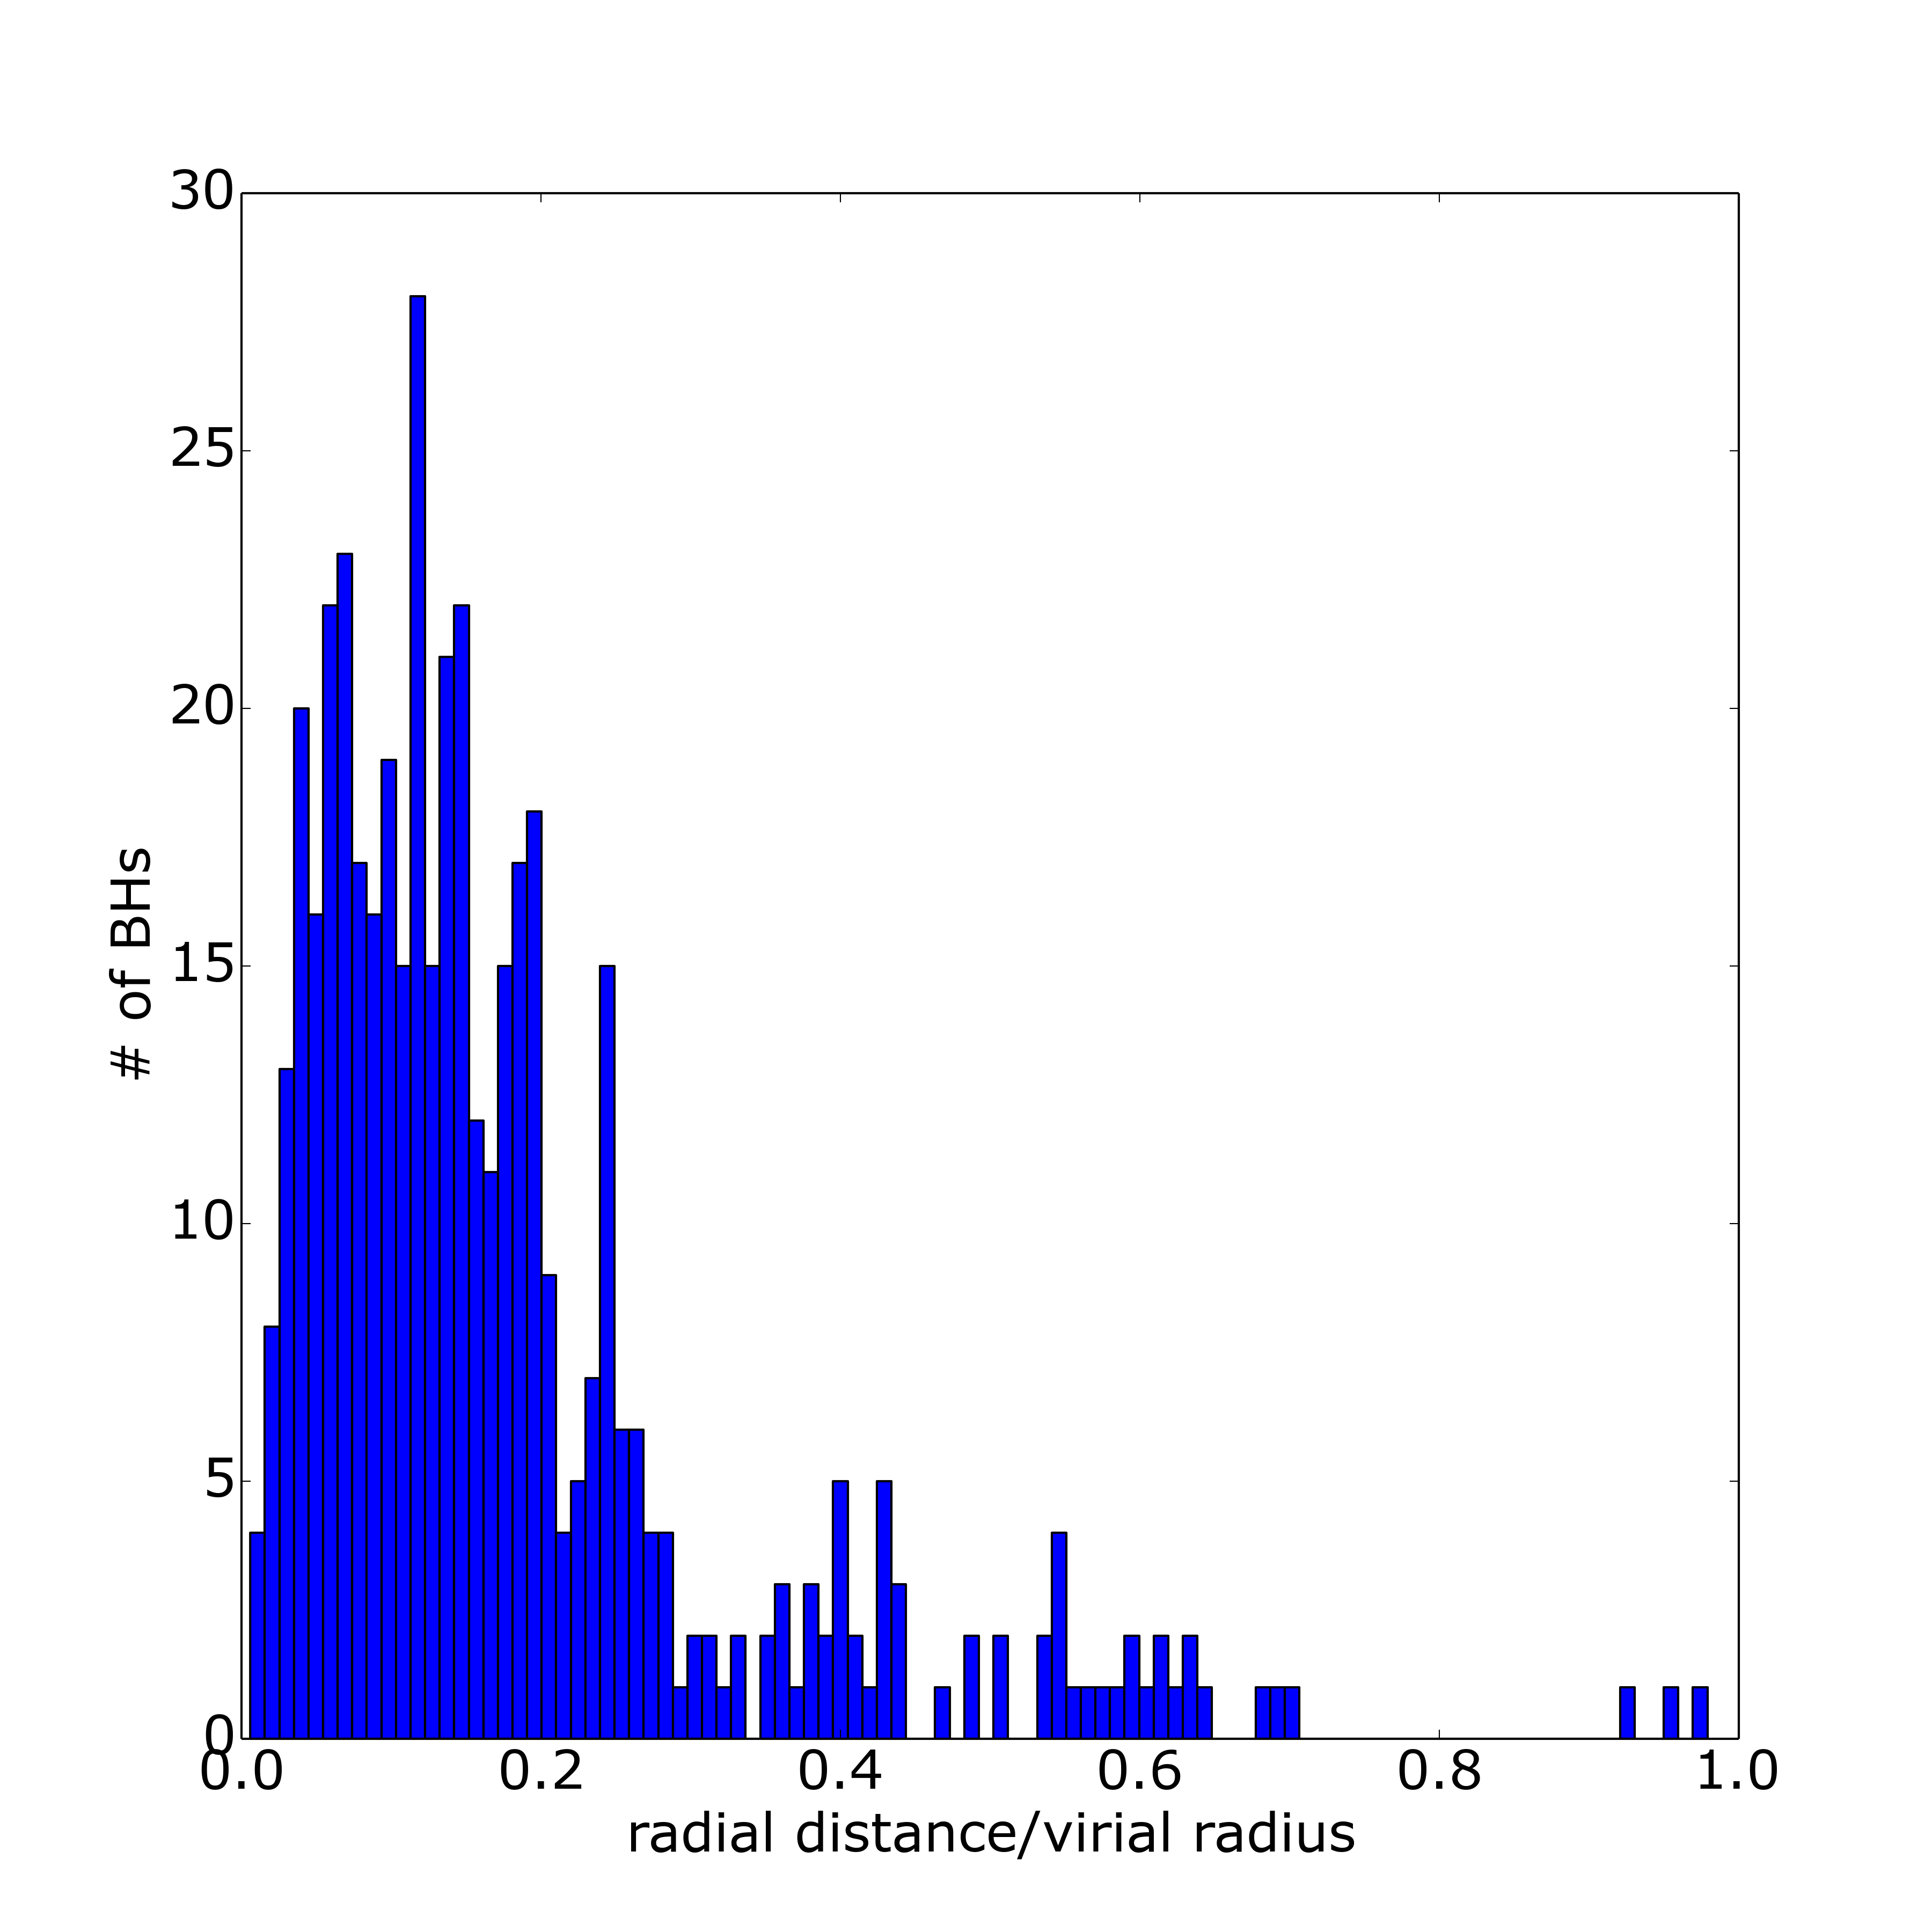
\includegraphics[keepaspectratio=true,width=0.8\linewidth]{rad_dist3.png}
%}
%\end{minipage}
%\begin{figure}
%  \centering
%  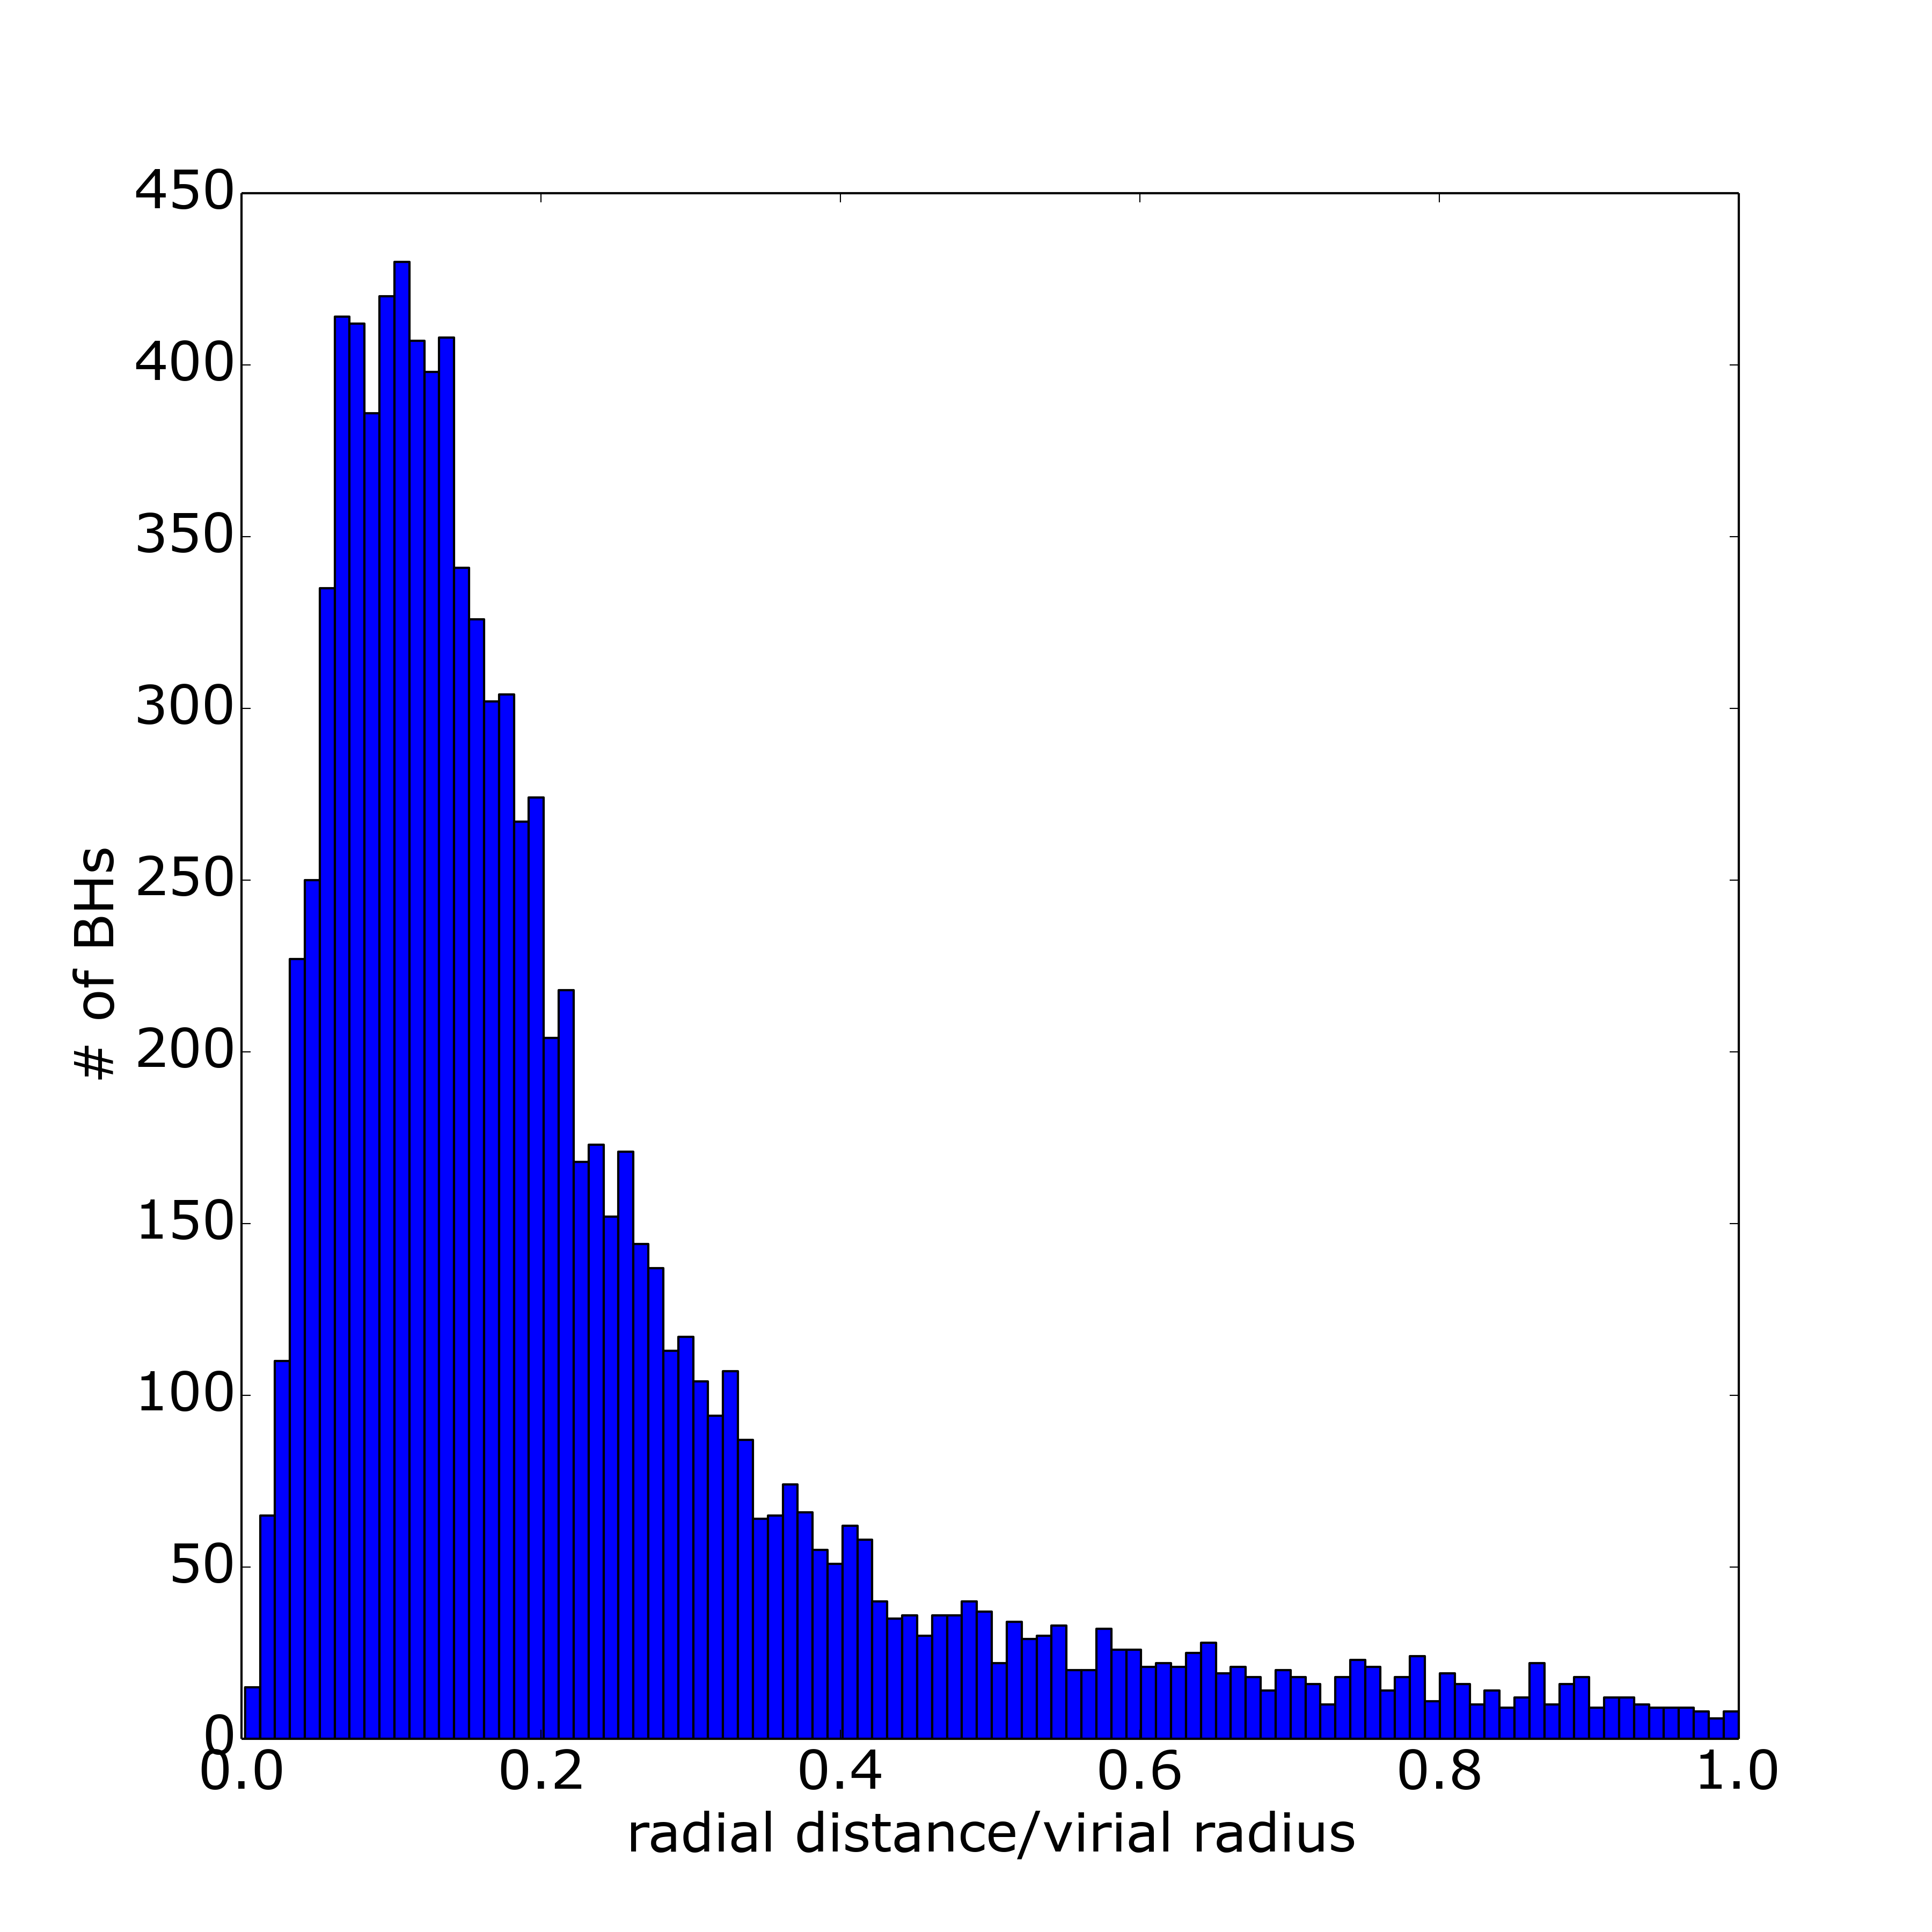
\includegraphics[width=0.8\columnwidth]{rad_dist14.png}
%\end{figure}
%\begin{figure}
%  \centering
%  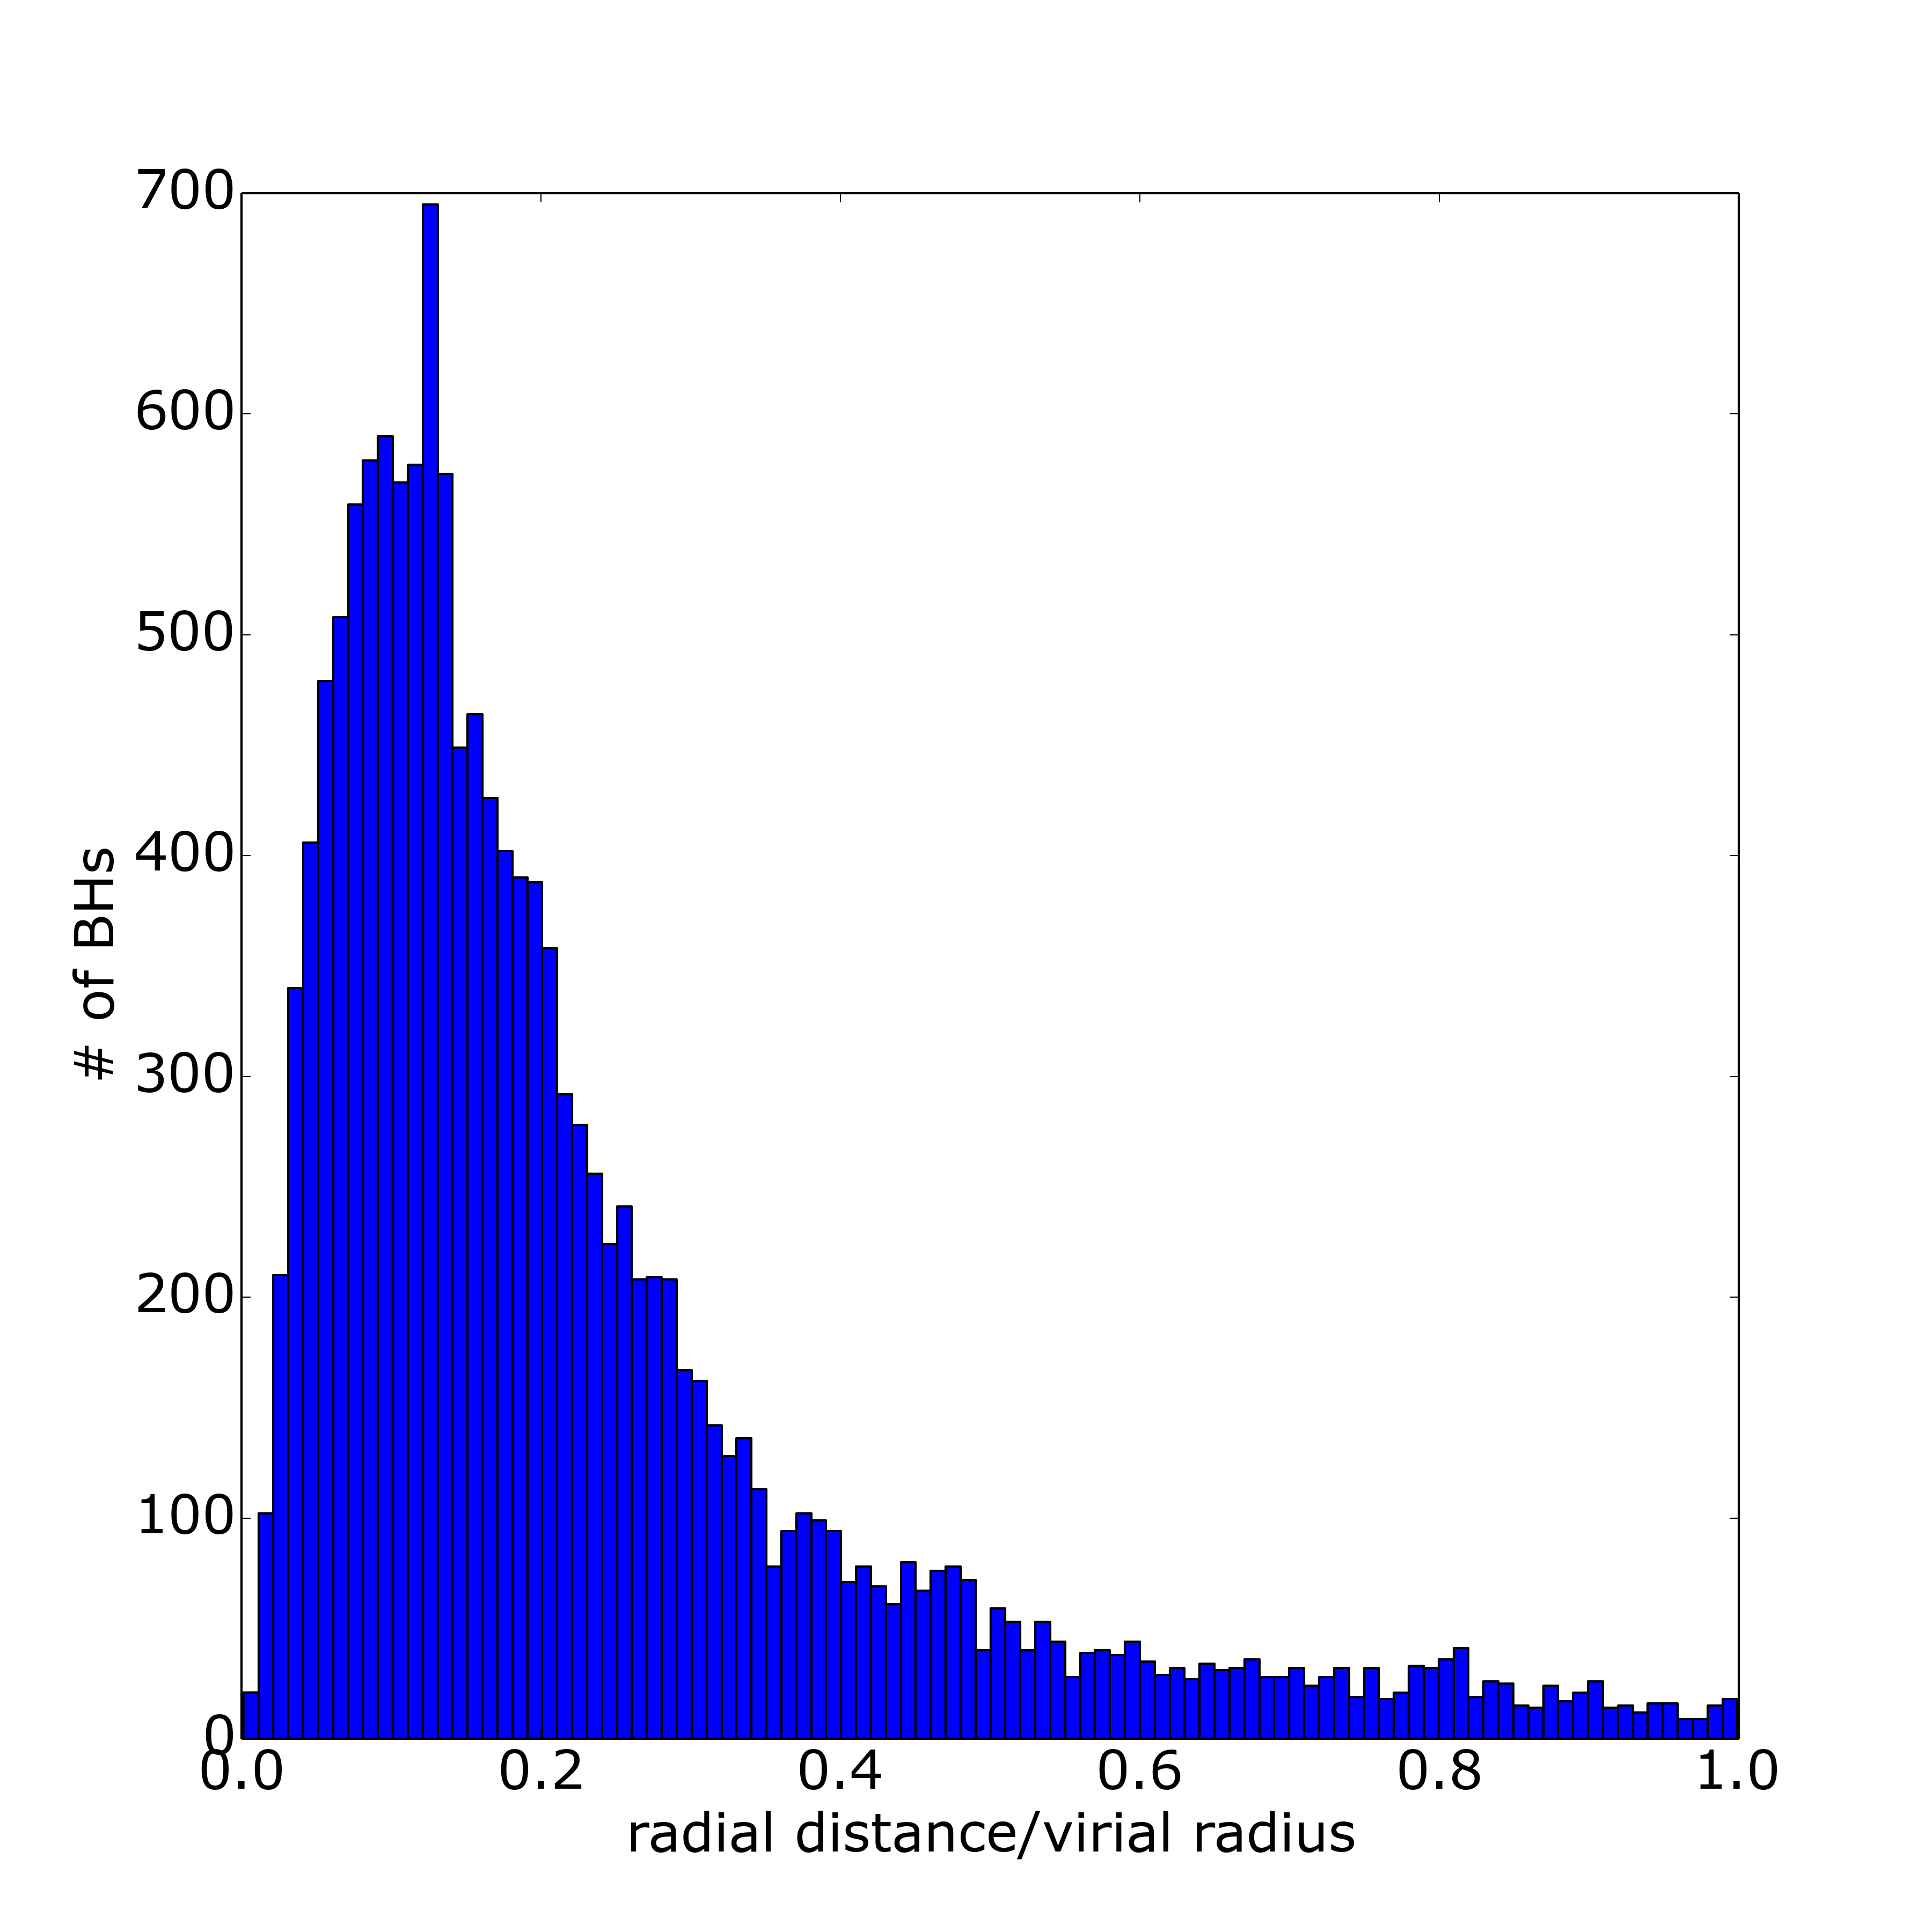
\includegraphics[width=0.8\columnwidth]{rad_dist22.png}
%\end{figure}
%Radial distribution of seed BHs of the final time step in different mass ranges:
%\begin{figure}
%  \centering
%  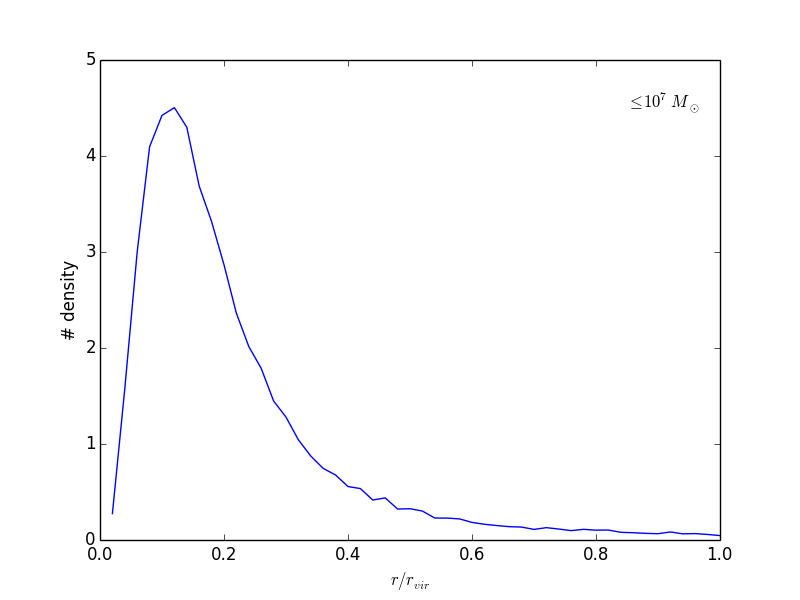
\includegraphics[width=0.8\columnwidth]{radist_mass7.png}
%\end{figure}
%
%\begin{figure}
%  \centering
%  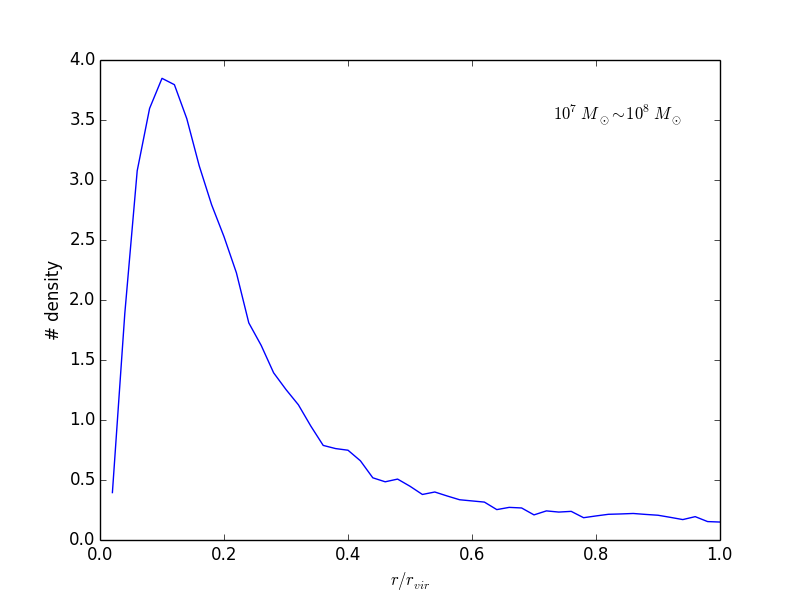
\includegraphics[width=0.8\columnwidth]{radist_mass8.png}
%\end{figure}
%
%\begin{figure}
%  \centering
%  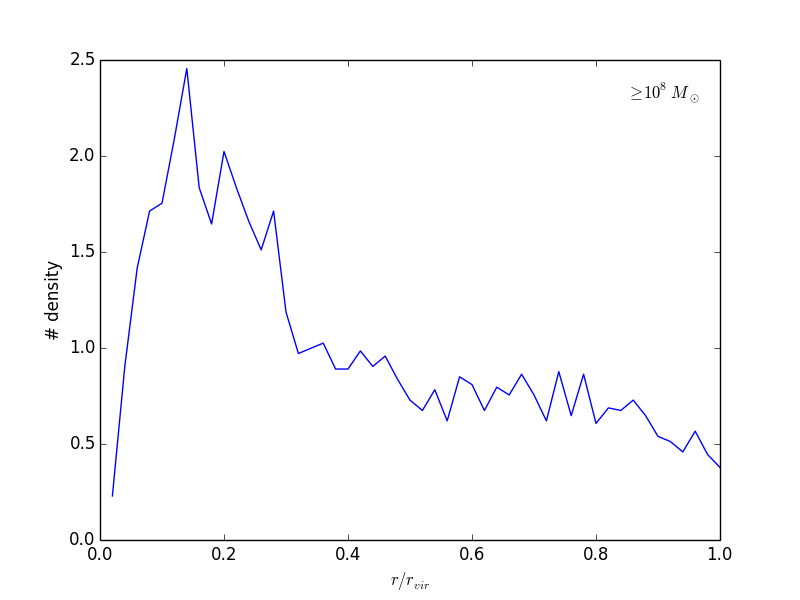
\includegraphics[width=0.8\columnwidth]{radist_mass9.png}
%\end{figure}

Orbital properties:
%\begin{figure}
%  \centering
%  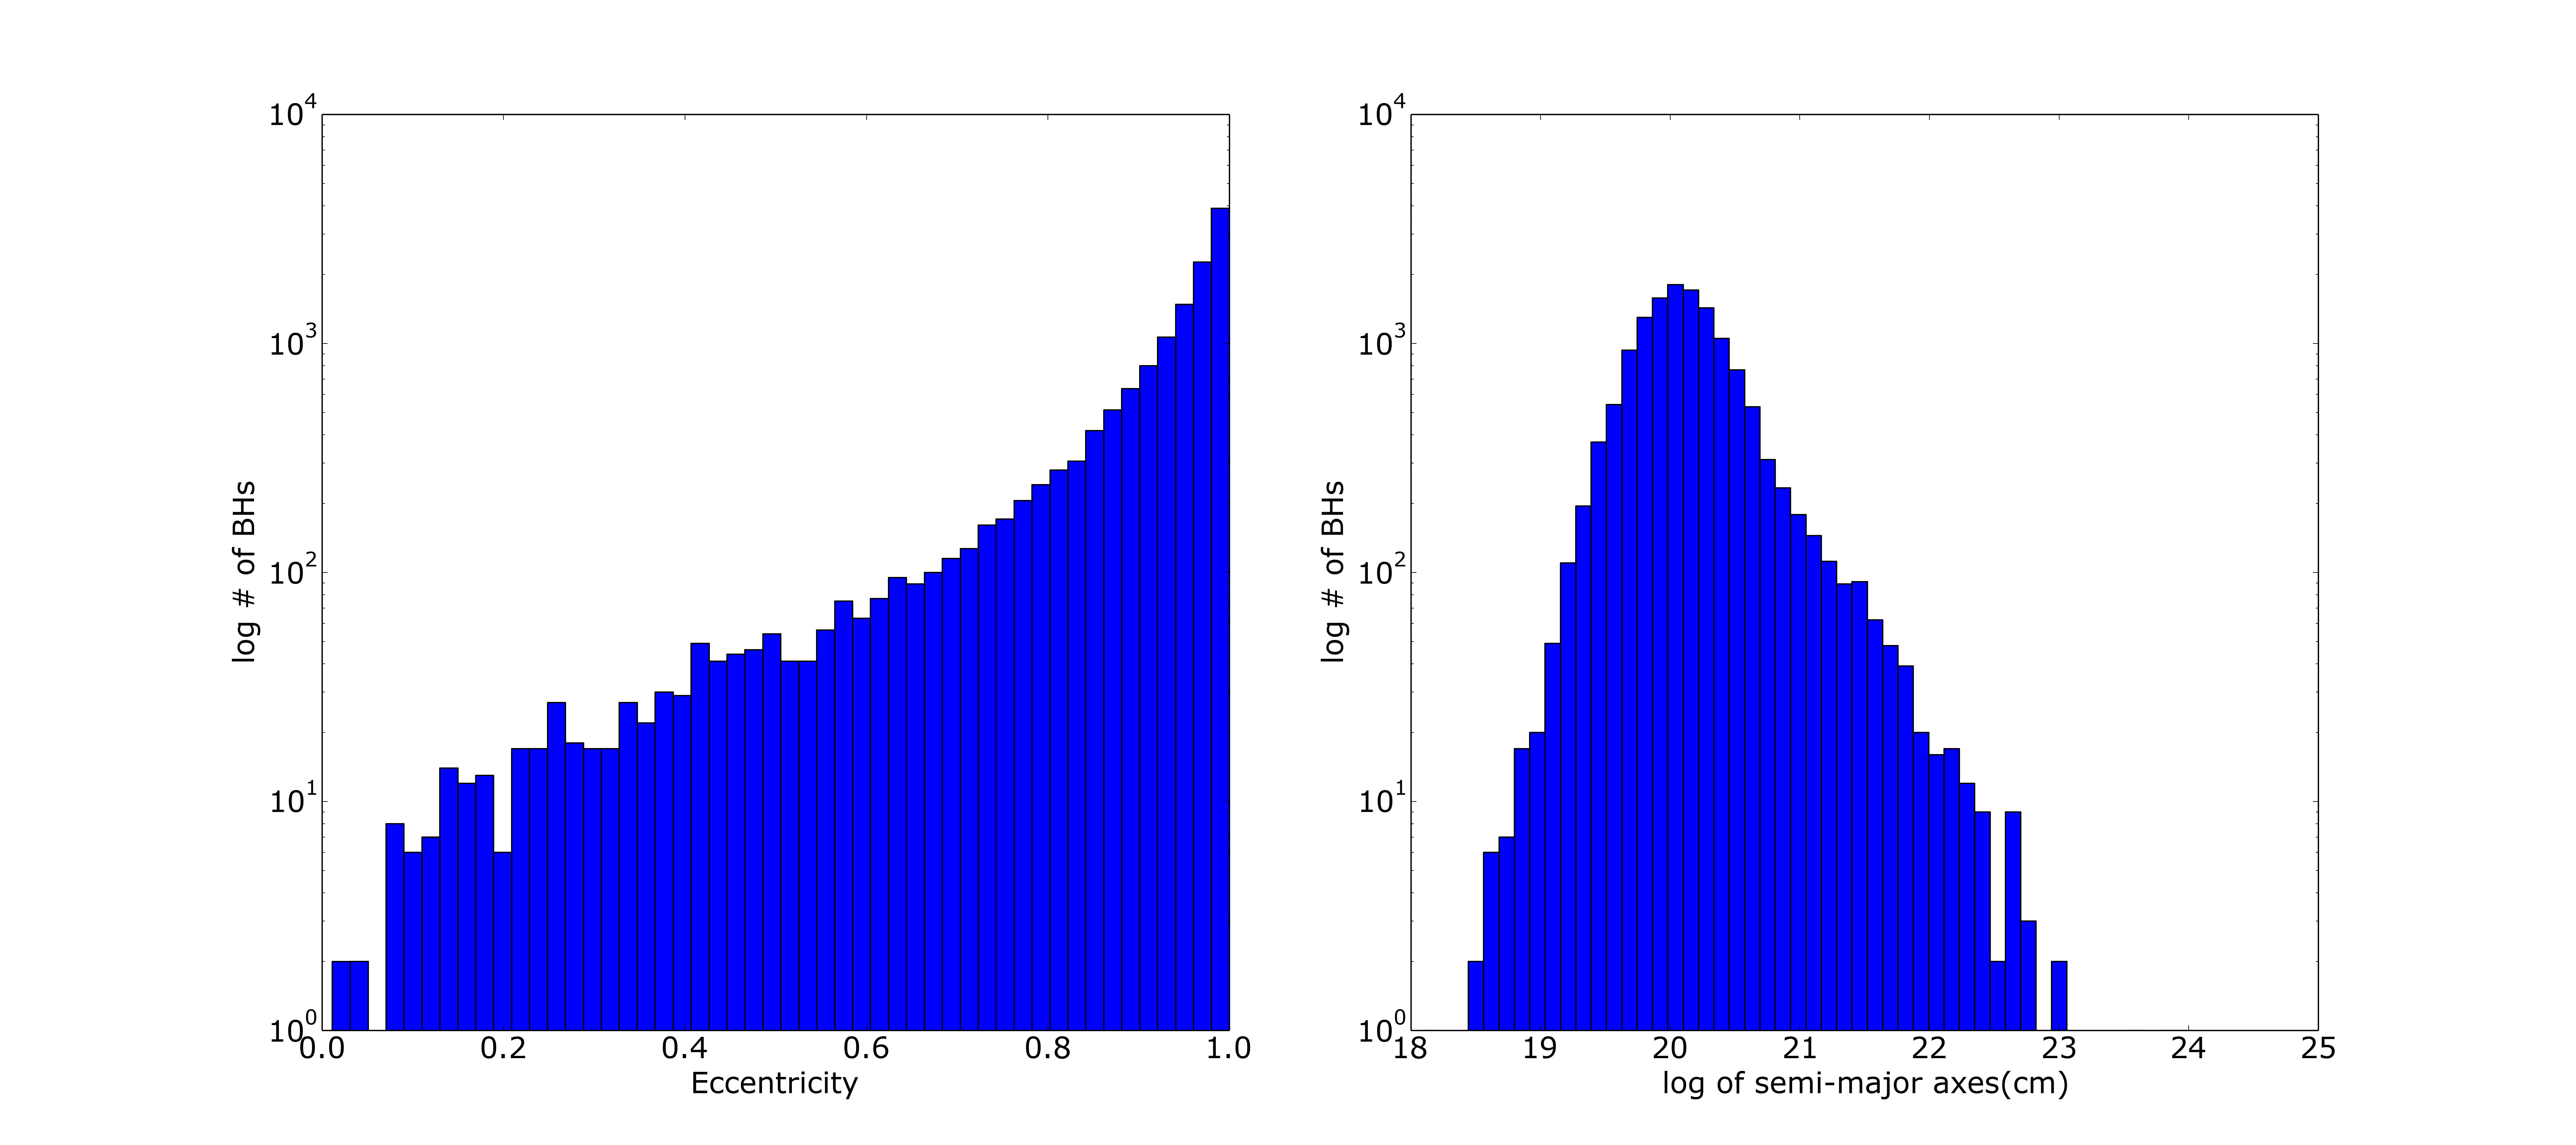
\includegraphics[width=0.8\columnwidth]{bhsorb_new.png}
%\end{figure}
%


\subsection{Case Study: High Temporal Analysis of a Single Galaxy}

Seed BHs position:
%\begin{figure}
%  \centering
%  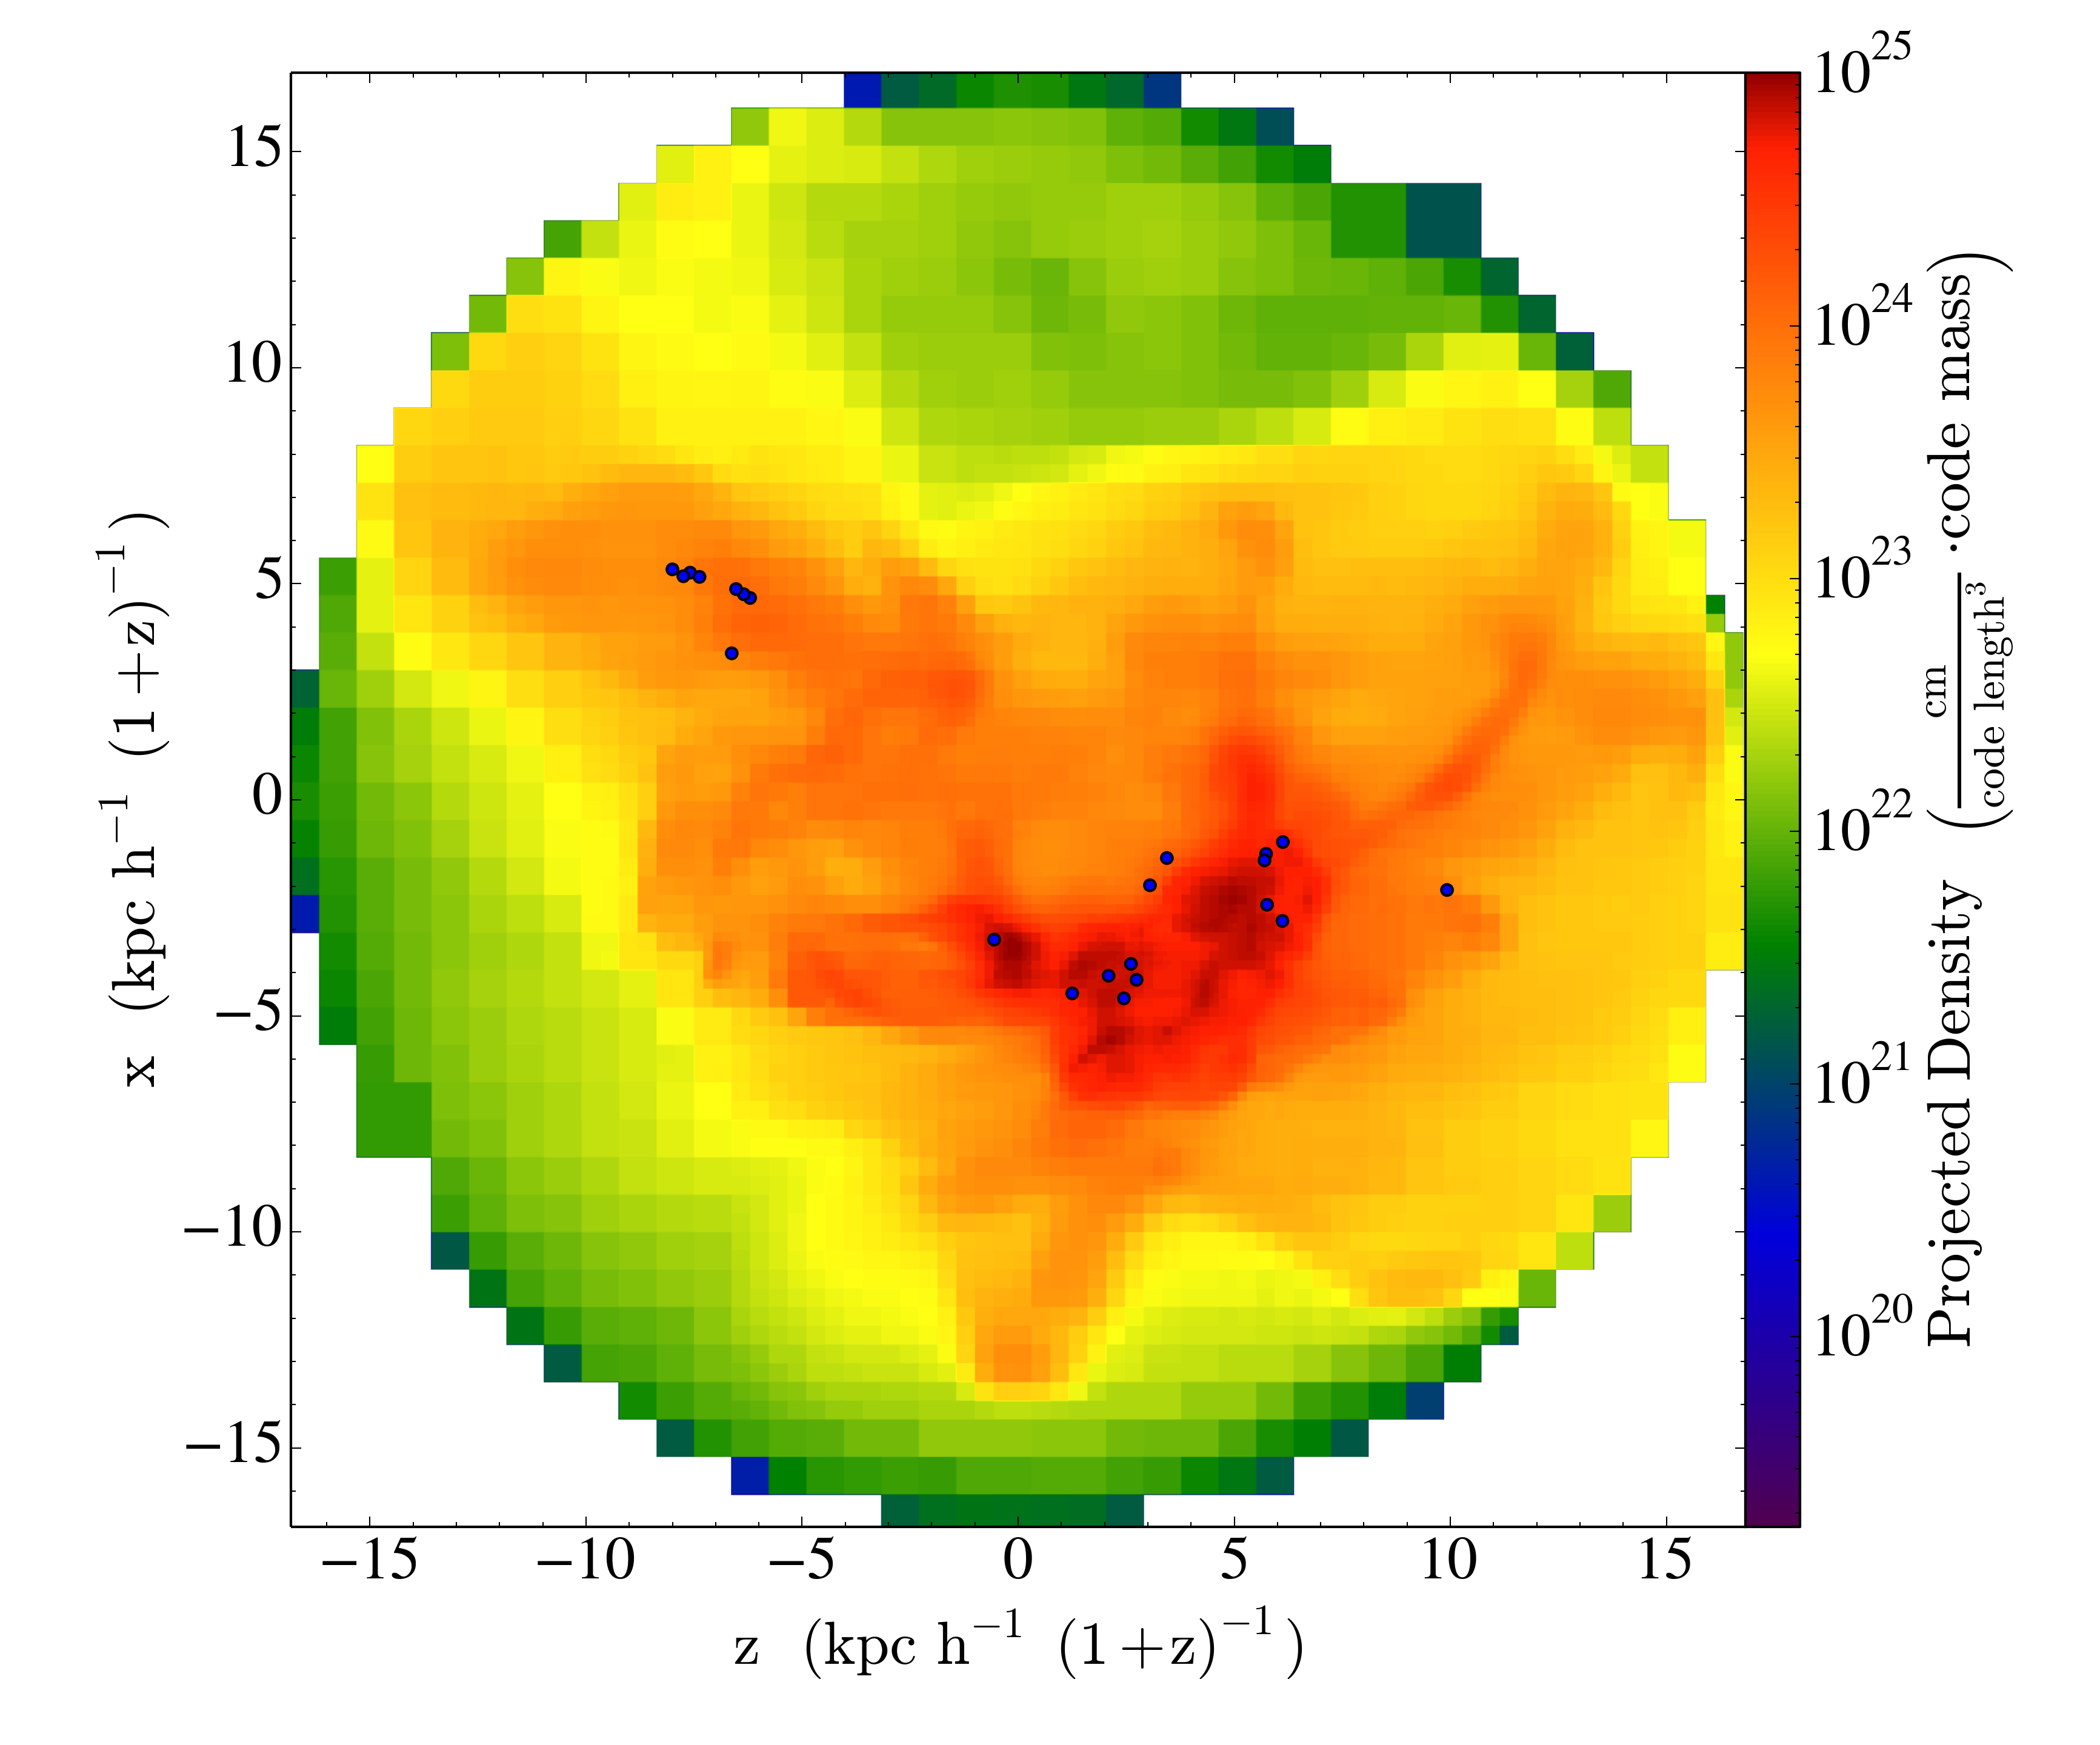
\includegraphics[width=0.8\columnwidth]{P0173_y_D.png}
%\end{figure}
%
%\begin{figure}
%  \centering
%  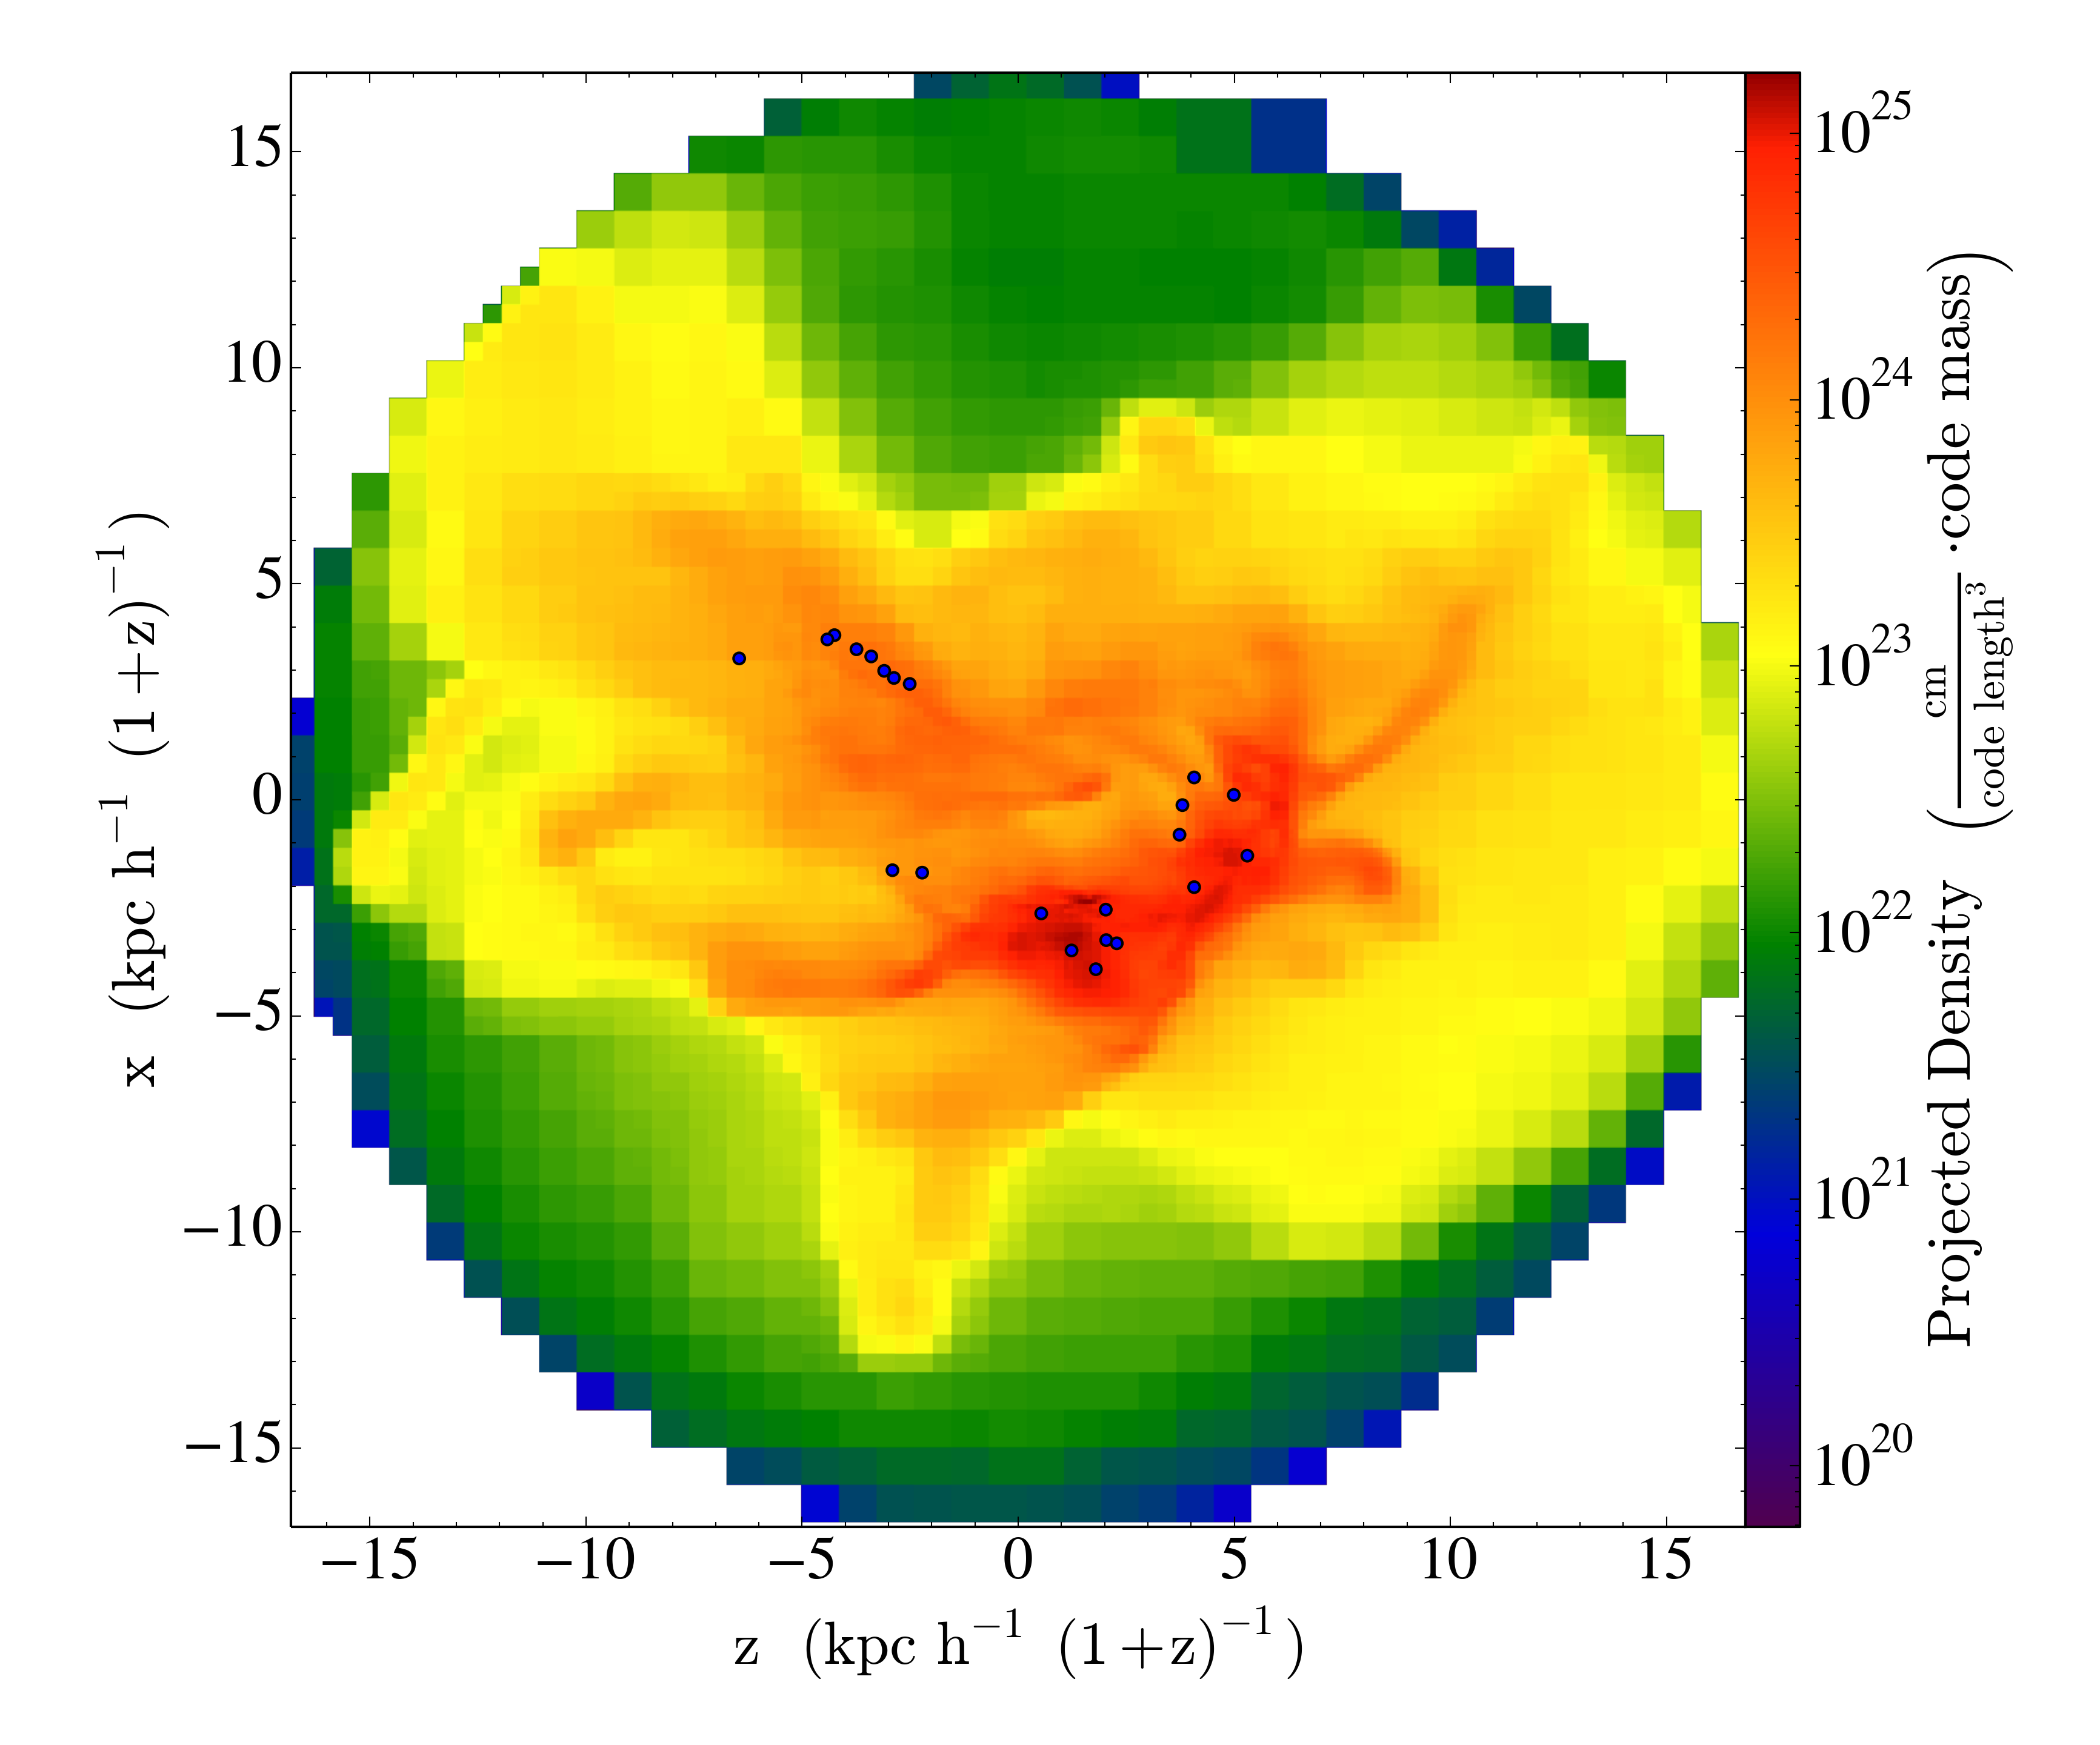
\includegraphics[width=0.8\columnwidth]{P0224_y_D.png}
%\end{figure}
%
%\begin{figure}
%  \centering
%  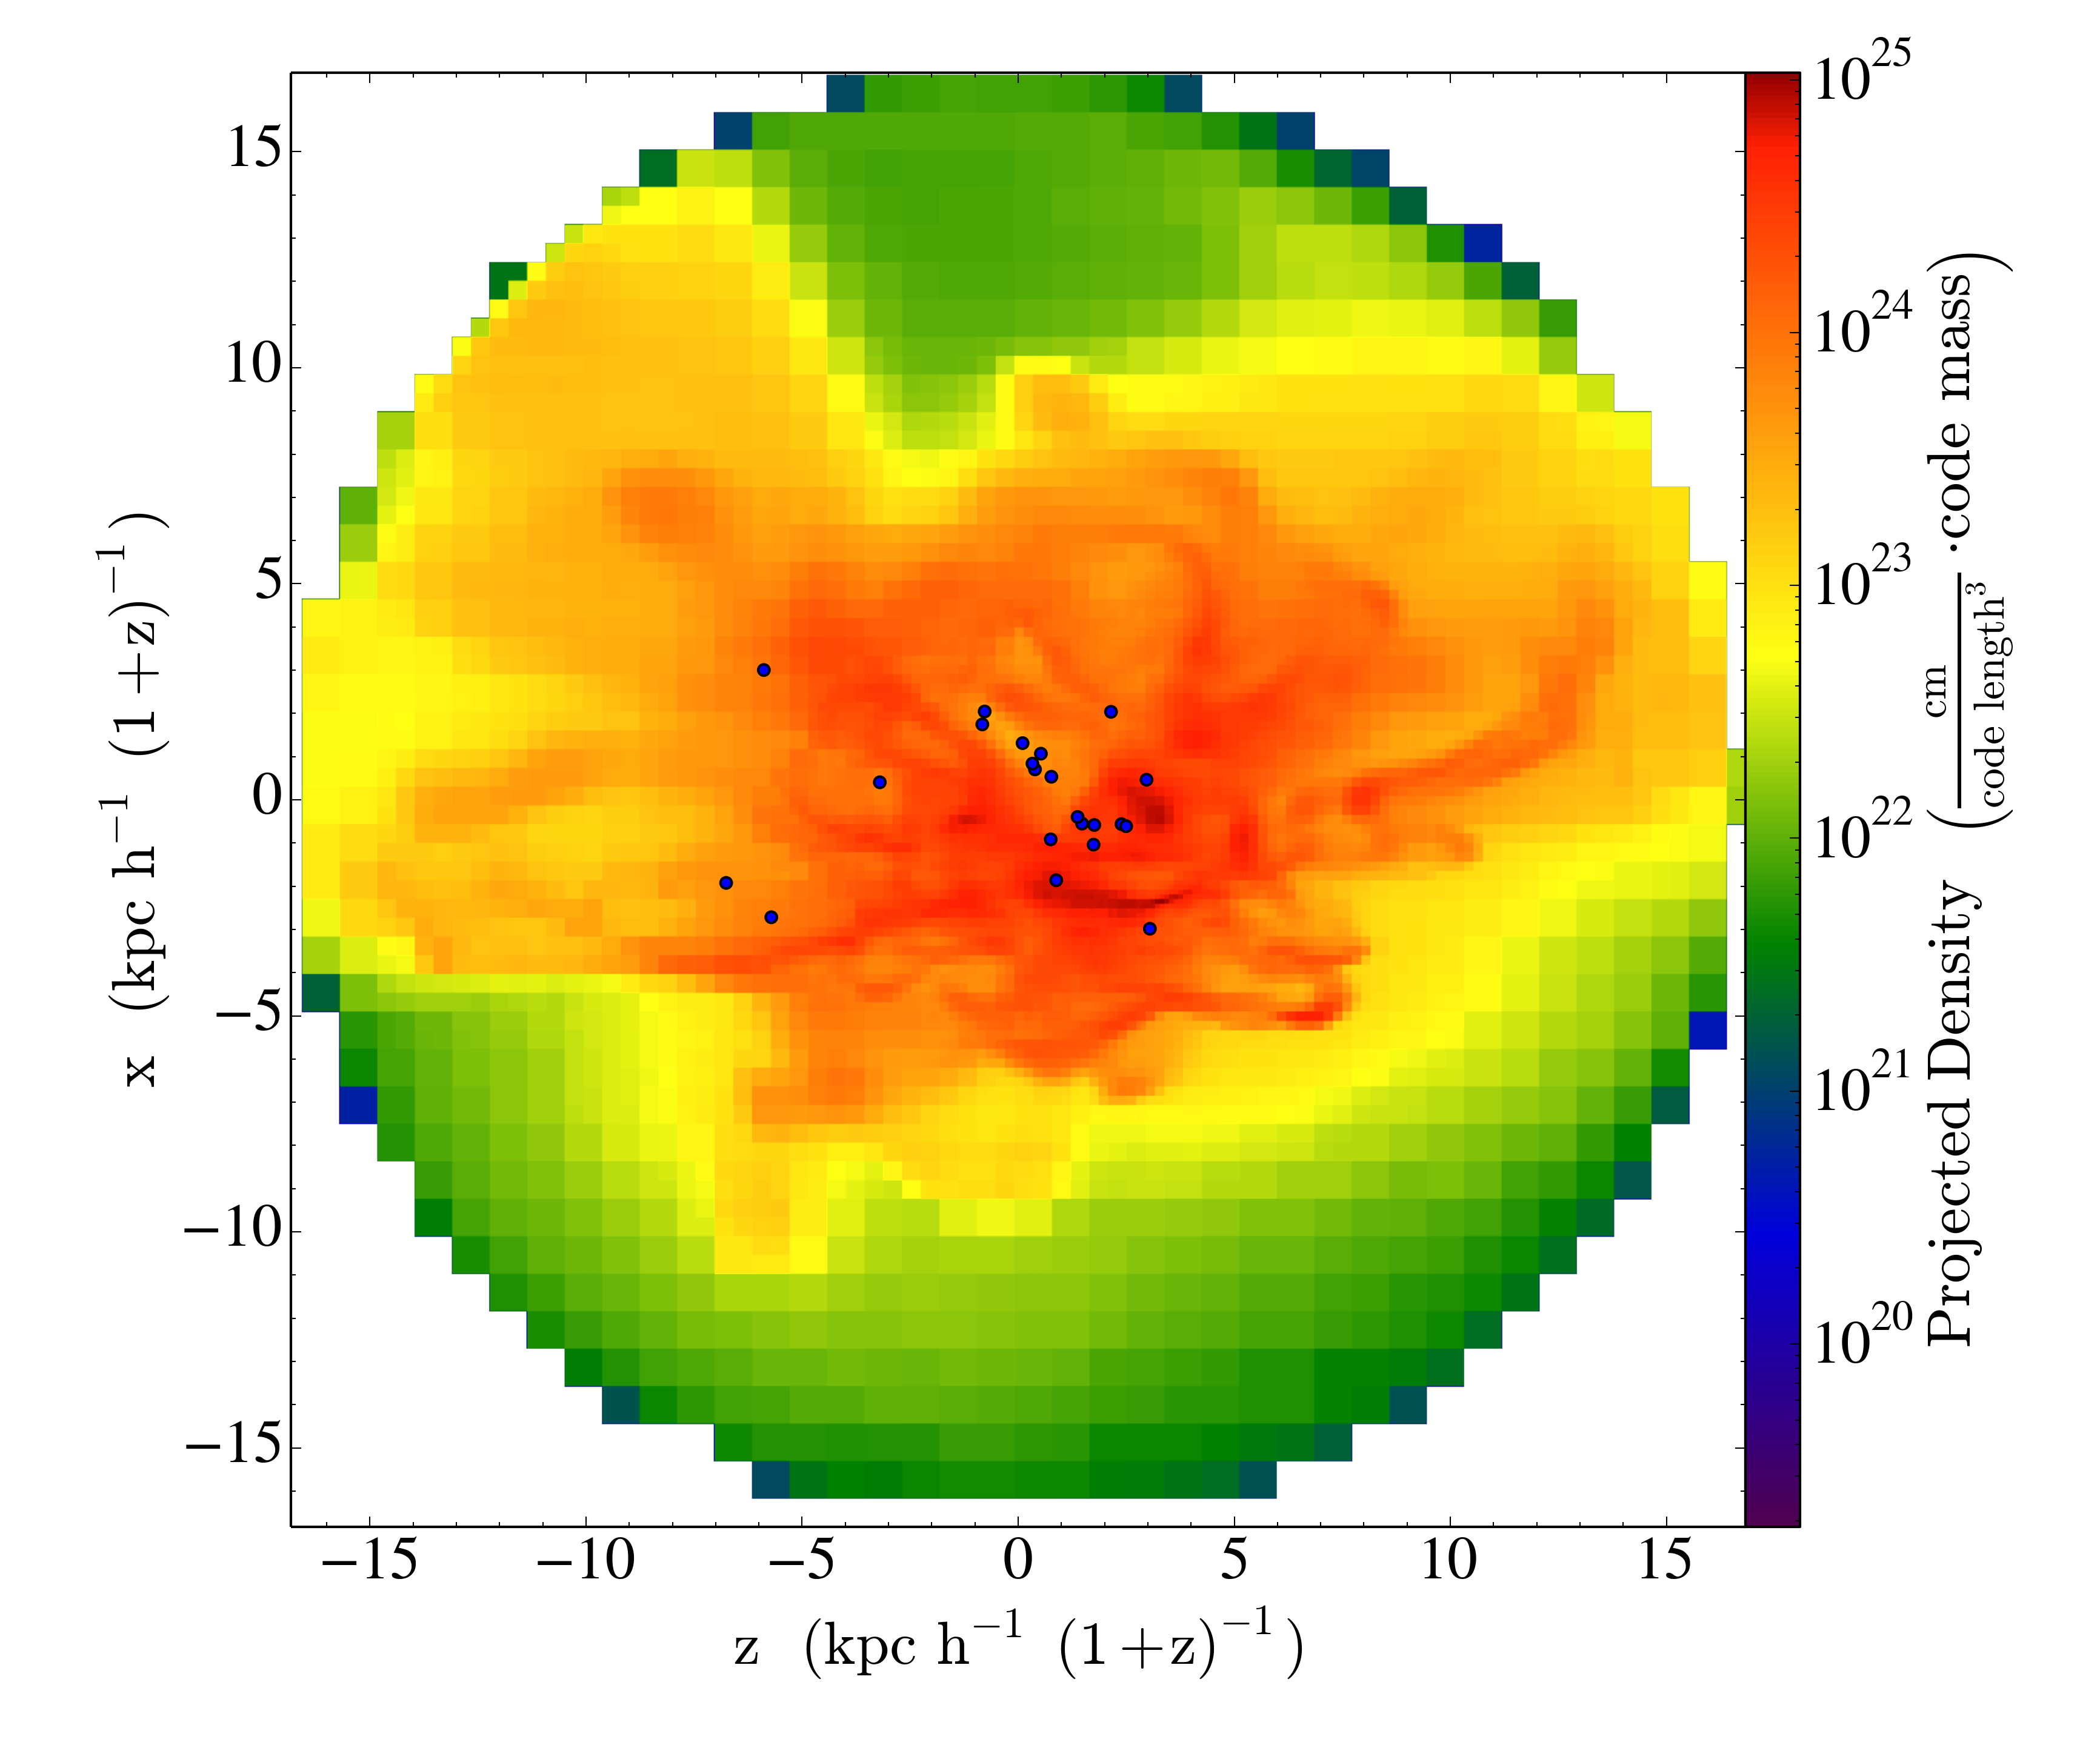
\includegraphics[width=0.8\columnwidth]{P0274_y_D.png}
%\end{figure}
Angular momentum evolution:

%\begin{figure}
%  \centering
%  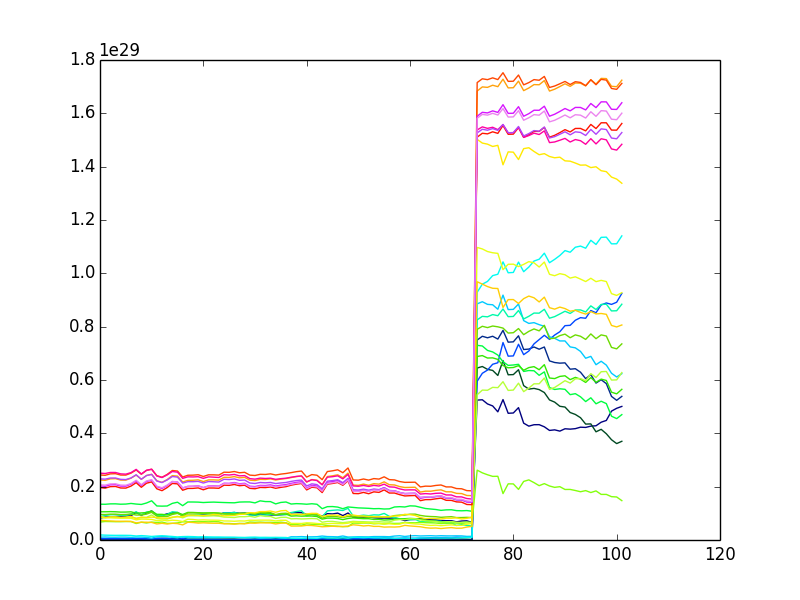
\includegraphics[width=0.8\columnwidth]{L2.png}
%\end{figure}


\section*{Acknowledgments}

This work is supported by NSF grants AST-1211626 and AST-1333360.
This research has made use of NASA's Astrophysics Data System
Bibliographic Services.  The majority of the analysis and plots were
done with \yt \citep{yt_full_paper}.

\bibliography{jwise}
\bsp
\label{lastpage}

\end{document}
